\documentclass[tikz,border=4pt]{standalone}
\usepackage{amsmath,amssymb}
\usetikzlibrary{arrows.meta}
\begin{document}
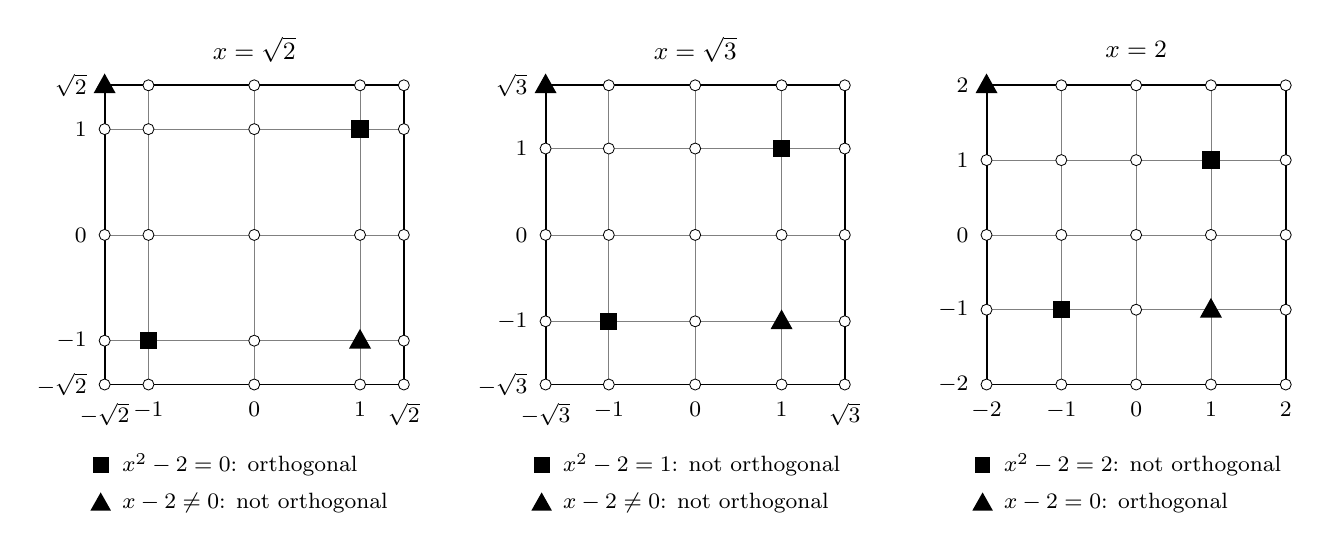
\begin{tikzpicture}[line cap=round,line join=round]
\draw[line width=0.7pt] (-1.9000,-1.9000) -- (-1.9000,1.9000);
\draw[line width=0.7pt] (-1.9000,-1.9000) -- (1.9000,-1.9000);
\draw[line width=0.3pt,gray] (-1.3435,-1.9000) -- (-1.3435,1.9000);
\draw[line width=0.3pt,gray] (-1.9000,-1.3435) -- (1.9000,-1.3435);
\draw[line width=0.3pt,gray] (0.0000,-1.9000) -- (0.0000,1.9000);
\draw[line width=0.3pt,gray] (-1.9000,0.0000) -- (1.9000,0.0000);
\draw[line width=0.3pt,gray] (1.3435,-1.9000) -- (1.3435,1.9000);
\draw[line width=0.3pt,gray] (-1.9000,1.3435) -- (1.9000,1.3435);
\draw[line width=0.7pt] (1.9000,-1.9000) -- (1.9000,1.9000);
\draw[line width=0.7pt] (-1.9000,1.9000) -- (1.9000,1.9000);
\draw[fill=white,line width=0.3pt] (-1.9000,-1.9000) circle (0.070);
\draw[fill=white,line width=0.3pt] (-1.9000,-1.3435) circle (0.070);
\draw[fill=white,line width=0.3pt] (-1.9000,0.0000) circle (0.070);
\draw[fill=white,line width=0.3pt] (-1.9000,1.3435) circle (0.070);
\fill (-2.0400,1.8000) -- (-1.7600,1.8000) -- (-1.9000,2.0500) -- cycle;
\draw[fill=white,line width=0.3pt] (-1.3435,-1.9000) circle (0.070);
\fill (-1.4535,-1.4535) rectangle (-1.2335,-1.2335);
\draw[fill=white,line width=0.3pt] (-1.3435,0.0000) circle (0.070);
\draw[fill=white,line width=0.3pt] (-1.3435,1.3435) circle (0.070);
\draw[fill=white,line width=0.3pt] (-1.3435,1.9000) circle (0.070);
\draw[fill=white,line width=0.3pt] (0.0000,-1.9000) circle (0.070);
\draw[fill=white,line width=0.3pt] (0.0000,-1.3435) circle (0.070);
\draw[fill=white,line width=0.3pt] (0.0000,0.0000) circle (0.070);
\draw[fill=white,line width=0.3pt] (0.0000,1.3435) circle (0.070);
\draw[fill=white,line width=0.3pt] (0.0000,1.9000) circle (0.070);
\draw[fill=white,line width=0.3pt] (1.3435,-1.9000) circle (0.070);
\fill (1.2035,-1.4435) -- (1.4835,-1.4435) -- (1.3435,-1.1935) -- cycle;
\draw[fill=white,line width=0.3pt] (1.3435,0.0000) circle (0.070);
\fill (1.2335,1.2335) rectangle (1.4535,1.4535);
\draw[fill=white,line width=0.3pt] (1.3435,1.9000) circle (0.070);
\draw[fill=white,line width=0.3pt] (1.9000,-1.9000) circle (0.070);
\draw[fill=white,line width=0.3pt] (1.9000,-1.3435) circle (0.070);
\draw[fill=white,line width=0.3pt] (1.9000,0.0000) circle (0.070);
\draw[fill=white,line width=0.3pt] (1.9000,1.3435) circle (0.070);
\draw[fill=white,line width=0.3pt] (1.9000,1.9000) circle (0.070);
\node[below=3pt,font=\footnotesize] at (-1.9000,-1.9000) {$-\sqrt2$};
\node[left=3pt,font=\footnotesize] at (-1.9000,-1.9000) {$-\sqrt2$};
\node[below=3pt,font=\footnotesize] at (-1.3435,-1.9000) {$-1$};
\node[left=3pt,font=\footnotesize] at (-1.9000,-1.3435) {$-1$};
\node[below=3pt,font=\footnotesize] at (0.0000,-1.9000) {$0$};
\node[left=3pt,font=\footnotesize] at (-1.9000,0.0000) {$0$};
\node[below=3pt,font=\footnotesize] at (1.3435,-1.9000) {$1$};
\node[left=3pt,font=\footnotesize] at (-1.9000,1.3435) {$1$};
\node[below=3pt,font=\footnotesize] at (1.9000,-1.9000) {$\sqrt2$};
\node[left=3pt,font=\footnotesize] at (-1.9000,1.9000) {$\sqrt2$};
\node[font=\small] at (0.0000,2.3500) {$x=\sqrt2$};
\fill (-2.0500,-3.0200) rectangle (-1.8500,-2.8200);
\node[right,font=\footnotesize] at (-1.8000,-2.9200) {$x^2-2=0$: orthogonal};
\fill (-2.0800,-3.5000) -- (-1.8200,-3.5000) -- (-1.9500,-3.2700) -- cycle;
\node[right,font=\footnotesize] at (-1.8000,-3.4000) {$x-2\neq0$: not orthogonal};
\draw[line width=0.7pt] (3.7000,-1.9000) -- (3.7000,1.9000);
\draw[line width=0.7pt] (3.7000,-1.9000) -- (7.5000,-1.9000);
\draw[line width=0.3pt,gray] (4.5030,-1.9000) -- (4.5030,1.9000);
\draw[line width=0.3pt,gray] (3.7000,-1.0970) -- (7.5000,-1.0970);
\draw[line width=0.3pt,gray] (5.6000,-1.9000) -- (5.6000,1.9000);
\draw[line width=0.3pt,gray] (3.7000,0.0000) -- (7.5000,0.0000);
\draw[line width=0.3pt,gray] (6.6970,-1.9000) -- (6.6970,1.9000);
\draw[line width=0.3pt,gray] (3.7000,1.0970) -- (7.5000,1.0970);
\draw[line width=0.7pt] (7.5000,-1.9000) -- (7.5000,1.9000);
\draw[line width=0.7pt] (3.7000,1.9000) -- (7.5000,1.9000);
\draw[fill=white,line width=0.3pt] (3.7000,-1.9000) circle (0.070);
\draw[fill=white,line width=0.3pt] (3.7000,-1.0970) circle (0.070);
\draw[fill=white,line width=0.3pt] (3.7000,0.0000) circle (0.070);
\draw[fill=white,line width=0.3pt] (3.7000,1.0970) circle (0.070);
\fill (3.5600,1.8000) -- (3.8400,1.8000) -- (3.7000,2.0500) -- cycle;
\draw[fill=white,line width=0.3pt] (4.5030,-1.9000) circle (0.070);
\fill (4.3930,-1.2070) rectangle (4.6130,-0.9870);
\draw[fill=white,line width=0.3pt] (4.5030,0.0000) circle (0.070);
\draw[fill=white,line width=0.3pt] (4.5030,1.0970) circle (0.070);
\draw[fill=white,line width=0.3pt] (4.5030,1.9000) circle (0.070);
\draw[fill=white,line width=0.3pt] (5.6000,-1.9000) circle (0.070);
\draw[fill=white,line width=0.3pt] (5.6000,-1.0970) circle (0.070);
\draw[fill=white,line width=0.3pt] (5.6000,0.0000) circle (0.070);
\draw[fill=white,line width=0.3pt] (5.6000,1.0970) circle (0.070);
\draw[fill=white,line width=0.3pt] (5.6000,1.9000) circle (0.070);
\draw[fill=white,line width=0.3pt] (6.6970,-1.9000) circle (0.070);
\fill (6.5570,-1.1970) -- (6.8370,-1.1970) -- (6.6970,-0.9470) -- cycle;
\draw[fill=white,line width=0.3pt] (6.6970,0.0000) circle (0.070);
\fill (6.5870,0.9870) rectangle (6.8070,1.2070);
\draw[fill=white,line width=0.3pt] (6.6970,1.9000) circle (0.070);
\draw[fill=white,line width=0.3pt] (7.5000,-1.9000) circle (0.070);
\draw[fill=white,line width=0.3pt] (7.5000,-1.0970) circle (0.070);
\draw[fill=white,line width=0.3pt] (7.5000,0.0000) circle (0.070);
\draw[fill=white,line width=0.3pt] (7.5000,1.0970) circle (0.070);
\draw[fill=white,line width=0.3pt] (7.5000,1.9000) circle (0.070);
\node[below=3pt,font=\footnotesize] at (3.7000,-1.9000) {$-\sqrt3$};
\node[left=3pt,font=\footnotesize] at (3.7000,-1.9000) {$-\sqrt3$};
\node[below=3pt,font=\footnotesize] at (4.5030,-1.9000) {$-1$};
\node[left=3pt,font=\footnotesize] at (3.7000,-1.0970) {$-1$};
\node[below=3pt,font=\footnotesize] at (5.6000,-1.9000) {$0$};
\node[left=3pt,font=\footnotesize] at (3.7000,0.0000) {$0$};
\node[below=3pt,font=\footnotesize] at (6.6970,-1.9000) {$1$};
\node[left=3pt,font=\footnotesize] at (3.7000,1.0970) {$1$};
\node[below=3pt,font=\footnotesize] at (7.5000,-1.9000) {$\sqrt3$};
\node[left=3pt,font=\footnotesize] at (3.7000,1.9000) {$\sqrt3$};
\node[font=\small] at (5.6000,2.3500) {$x=\sqrt3$};
\fill (3.5500,-3.0200) rectangle (3.7500,-2.8200);
\node[right,font=\footnotesize] at (3.8000,-2.9200) {$x^2-2=1$: not orthogonal};
\fill (3.5200,-3.5000) -- (3.7800,-3.5000) -- (3.6500,-3.2700) -- cycle;
\node[right,font=\footnotesize] at (3.8000,-3.4000) {$x-2\neq0$: not orthogonal};
\draw[line width=0.7pt] (9.3000,-1.9000) -- (9.3000,1.9000);
\draw[line width=0.7pt] (9.3000,-1.9000) -- (13.1000,-1.9000);
\draw[line width=0.3pt,gray] (10.2500,-1.9000) -- (10.2500,1.9000);
\draw[line width=0.3pt,gray] (9.3000,-0.9500) -- (13.1000,-0.9500);
\draw[line width=0.3pt,gray] (11.2000,-1.9000) -- (11.2000,1.9000);
\draw[line width=0.3pt,gray] (9.3000,0.0000) -- (13.1000,0.0000);
\draw[line width=0.3pt,gray] (12.1500,-1.9000) -- (12.1500,1.9000);
\draw[line width=0.3pt,gray] (9.3000,0.9500) -- (13.1000,0.9500);
\draw[line width=0.7pt] (13.1000,-1.9000) -- (13.1000,1.9000);
\draw[line width=0.7pt] (9.3000,1.9000) -- (13.1000,1.9000);
\draw[fill=white,line width=0.3pt] (9.3000,-1.9000) circle (0.070);
\draw[fill=white,line width=0.3pt] (9.3000,-0.9500) circle (0.070);
\draw[fill=white,line width=0.3pt] (9.3000,0.0000) circle (0.070);
\draw[fill=white,line width=0.3pt] (9.3000,0.9500) circle (0.070);
\fill (9.1600,1.8000) -- (9.4400,1.8000) -- (9.3000,2.0500) -- cycle;
\draw[fill=white,line width=0.3pt] (10.2500,-1.9000) circle (0.070);
\fill (10.1400,-1.0600) rectangle (10.3600,-0.8400);
\draw[fill=white,line width=0.3pt] (10.2500,0.0000) circle (0.070);
\draw[fill=white,line width=0.3pt] (10.2500,0.9500) circle (0.070);
\draw[fill=white,line width=0.3pt] (10.2500,1.9000) circle (0.070);
\draw[fill=white,line width=0.3pt] (11.2000,-1.9000) circle (0.070);
\draw[fill=white,line width=0.3pt] (11.2000,-0.9500) circle (0.070);
\draw[fill=white,line width=0.3pt] (11.2000,0.0000) circle (0.070);
\draw[fill=white,line width=0.3pt] (11.2000,0.9500) circle (0.070);
\draw[fill=white,line width=0.3pt] (11.2000,1.9000) circle (0.070);
\draw[fill=white,line width=0.3pt] (12.1500,-1.9000) circle (0.070);
\fill (12.0100,-1.0500) -- (12.2900,-1.0500) -- (12.1500,-0.8000) -- cycle;
\draw[fill=white,line width=0.3pt] (12.1500,0.0000) circle (0.070);
\fill (12.0400,0.8400) rectangle (12.2600,1.0600);
\draw[fill=white,line width=0.3pt] (12.1500,1.9000) circle (0.070);
\draw[fill=white,line width=0.3pt] (13.1000,-1.9000) circle (0.070);
\draw[fill=white,line width=0.3pt] (13.1000,-0.9500) circle (0.070);
\draw[fill=white,line width=0.3pt] (13.1000,0.0000) circle (0.070);
\draw[fill=white,line width=0.3pt] (13.1000,0.9500) circle (0.070);
\draw[fill=white,line width=0.3pt] (13.1000,1.9000) circle (0.070);
\node[below=3pt,font=\footnotesize] at (9.3000,-1.9000) {$-2$};
\node[left=3pt,font=\footnotesize] at (9.3000,-1.9000) {$-2$};
\node[below=3pt,font=\footnotesize] at (10.2500,-1.9000) {$-1$};
\node[left=3pt,font=\footnotesize] at (9.3000,-0.9500) {$-1$};
\node[below=3pt,font=\footnotesize] at (11.2000,-1.9000) {$0$};
\node[left=3pt,font=\footnotesize] at (9.3000,0.0000) {$0$};
\node[below=3pt,font=\footnotesize] at (12.1500,-1.9000) {$1$};
\node[left=3pt,font=\footnotesize] at (9.3000,0.9500) {$1$};
\node[below=3pt,font=\footnotesize] at (13.1000,-1.9000) {$2$};
\node[left=3pt,font=\footnotesize] at (9.3000,1.9000) {$2$};
\node[font=\small] at (11.2000,2.3500) {$x=2$};
\fill (9.1500,-3.0200) rectangle (9.3500,-2.8200);
\node[right,font=\footnotesize] at (9.4000,-2.9200) {$x^2-2=2$: not orthogonal};
\fill (9.1200,-3.5000) -- (9.3800,-3.5000) -- (9.2500,-3.2700) -- cycle;
\node[right,font=\footnotesize] at (9.4000,-3.4000) {$x-2=0$: orthogonal};
\end{tikzpicture}
\end{document}
